% !TeX root = ../../main.tex
\chapter{图表记录}
\label{chap:chapter6}

\section{图表示例}
表\ref{tab:example}与图\ref{fig:example}仅为排版示例。
\begin{table}[htbp]
  \centering
  \caption{示例数据}\label{tab:example}
  \begin{tabular}{ccc}
    \toprule
    序号 & 输入 & 输出 \\
    \midrule
    1 & 1 & 2 \\
    2 & 2 & 4 \\
    3 & 3 & 6 \\
    \bottomrule
  \end{tabular}
\end{table}

\begin{figure}[htbp]
  \centering
  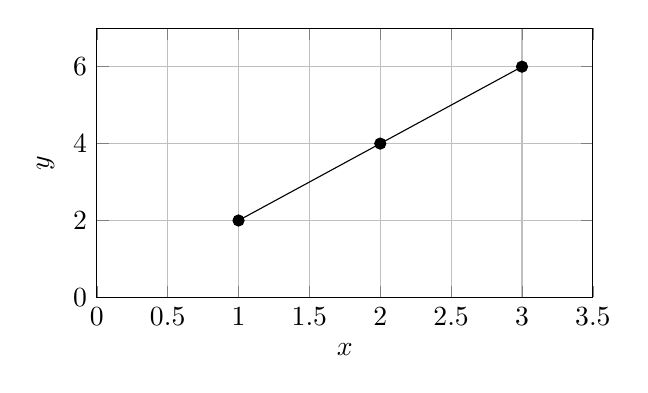
\begin{tikzpicture}
    \begin{axis}[
      width=0.65\linewidth,height=5cm,
      xlabel={$x$},ylabel={$y$},
      xmin=0,xmax=3.5,ymin=0,ymax=7,
      grid=major
    ]
      \addplot[black,mark=*] coordinates {(1,2) (2,4) (3,6)};
    \end{axis}
  \end{tikzpicture}
  \caption{示例关系 \(y=2x\)}\label{fig:example}
\end{figure}

\section{补充说明}
这里记录图表的说明。
